% !TeX root = main.tex
\lecture{15}{Tue 10 Mar 2026 12:00}{Statistical Physics II: The Atmosphere}

\section{The Atmosphere}
The very outer part of the atmosphere, from $90$km to $350$km is the ionosphere. This acts as a mirror which reflects EM radiation 

\begin{figure}[H]
    \centering
    
\includegraphics[width=0.75\textwidth]{figures/lec15-01.png}
     \caption{}
\end{figure}

This is how we're able to do international radio communications, by bouncing radio waves off of this layer in order to reach continents where there is no direct line of sight.

\subsection{Isothermal Model of the Atmosphere}
Consider an observer sitting in the troposphere above the earth, looking at a small cuboidal slice of the troposphere.

We will assume that:
\begin{itemize}
    \item The atmosphere is isothermal. In reality, increasing height reduces temperature by approx. $10$K per km.
    \item The atmosphere is solely comprised of an ideal gas. At the low pressure scales relevant for the atmosphere, this is a reasonable assumption.
    \item The earth is flat\footnote{Oh dear\dots}. Technically, assume that we we consider small enough heights and cross-sectional areas that we can disregard the curvature of the earth.
    \item The atmosphere is stationary and is therefore in mechanical equilibrium. This can be a good approximation depending on weather conditions.
\end{itemize}

The slab of atmosphere we're considering has area $A$, height $dh$ and sits at height $h$ above the surface of the earth. From the ideal gas state equation:
\[
    PV = \underbrace{nRT}_\text{moles} = \underbrace{N k_B T}_\text{particles}
\]
\[
    \implies P = \frac{N}{V} k_B T
\]
\[
    \implies P = \rho_N k_B T
\]

Where $\rho_N = N/V$ is number density, and is defined as the number of molecules per unit volume.

The slab of atmosphere has two forces acting upon it, a force due to pressure and a force due to gravity. As we assume that slice is in mechanical equilibrium, we can equate these forces.

The pressure is going to vary across the slab. Force due to pressure increases the further down into the atmosphere you go. This means the bottom face of the slab experiences a higher pressure than the top face. Since the slab is in mechanical equilibrium, the force due to gravity must balance the net upwards pressure force.

This gives us:
\[
    \text{force due to gravity } = \text{ force due to pressure}
\]
\[
    mg \rho_N V = A P(h) - A P(h + dh)
\]
\[
    mg \rho_N V = -d P(h) A
\]
\[
    mg \rho_N \times dh \times A = - d \rho(h) A
\]
\[
    mg \rho_N \times dh =  -d \rho(h)
\]
\[
    \frac{d \rho(h)}{dh} - mg \rho(N)
\]
\[
    \int d \rho(h) = - \int mg \rho_N dh
\]

And considering number density in the density integral:
\[
    \int_{\rho(0)}^{\rho(h)} \frac{1}{\rho_N} d \rho(h) = - \int_{0}^{h} mg dh
\]

And substituting $dp = d \rho_N k_B T$ to give a LHS integral entirely in number density:
\[
    \int_{\rho_N(0)}^{\rho_N(h)} \frac{k_B T}{\rho_N} d \rho_N = -mgh    
\]
\[
    \int_{\rho_N(0)}^{\rho_N(h)} \frac{k_B T}{\rho_N} d \rho_N = -\frac{mgh}{k_B T}   
\]
\[
    \left[\ln \left(\rho_N\right)\right]^{\rho_N(h)}_{\rho_N(0)} = -\frac{mgh}{k_B T}   
\]
\[
    \frac{\rho_N(h)}{\rho_N(0)} = \exp \left(- \frac{mgh}{k_B T}\right) \implies {\rho_N(h) = \rho_N(0) \exp \left(- \frac{mgh}{k_B T}\right)}
\]

The contents of the exponential have to be unitless, and they are because they're both units of energy. The upper gives gravitational energy, the lower gives thermal energy and the contents of the exponential depends on the ratio between the two of them.

This gives the final result:
\[
    \boxed{\rho_N(h) = \rho_N(0) \exp \left(- \frac{mgh}{k_B T}\right)}
\]
 
And as $P = \rho_n k_B T$:
\[
    {P(h) k_B T = P(0) k_B T \exp \left(- \frac{mgh}{k_B T}\right)}
\]
\[
    \implies \boxed{P(h) = P(0) \exp \left(- \frac{mgh}{k_B T}\right)}
\]

\begin{figure}[H]
    \centering
    
\includegraphics[width=0.75\textwidth]{figures/lec15-02.png}
     \caption{}
\end{figure}

\subsection{Scale Height}
As $mgh / k_B T$ must be dimensionless, $mg / k_B T$ must have units of $h$. We call this the scale height, $h_0$. This is the height at which $P(h_0) = P(0) e^{-1}$, i.e. the point at which pressure drops off by a factor of $1/e$.

\begin{figure}[H]
    \centering
    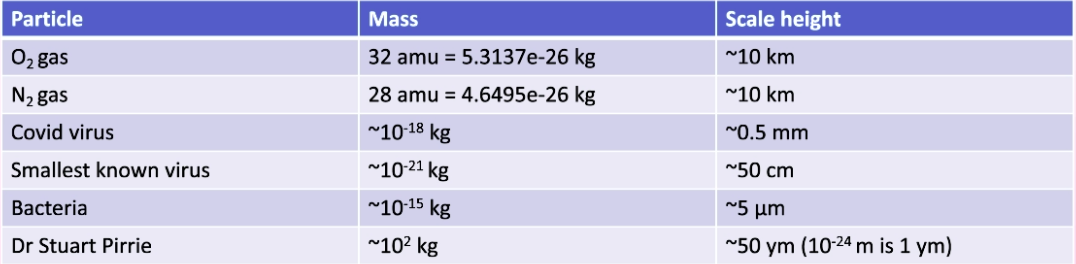
\includegraphics[width=\textwidth]{figures/lec15-03.png}
     \caption{Example Scale Heights}
\end{figure}

This helps answer the question ``if someone coughs on a desk, are other people in the room safe from Covid?''. This implies yes, as the scale heigh is much larger than anyone is likely to be above a desk. This isn't true for all viruses however, i.e. the $50$cm scale height for the smallest known virus.